\documentclass{beamer}
\usepackage{beamerthemesplit}
\usepackage{pgfgantt}
\usetheme{Warsaw}
\usecolortheme{wolverine}
\usepackage{sidecap}
%\usepackage[frenchb]{babel}
%\usepackage[latin1]{inputenc}
\usepackage[utf8x]{inputenc}
\usetikzlibrary{babel}
\usepackage{lmodern}
\usepackage[T1]{fontenc}
\usepackage{amsfonts}
\usepackage{amsmath,amssymb,theorem}
\usepackage[all]{xy}
\usepackage{textcomp}
\usepackage{pstricks,pst-plot,pstricks-add}
\usepackage{bm, listings, ccaption, mathrsfs}
\usepackage{xcolor,epic,eepic,multicol, colortbl}
\graphicspath{{Images_Fichiers/}}
\newcommand{\sg}[1]{\textbf{\underline{#1}}}
\newcommand{\e}[1]{\bm{e_{#1}}}
\newcommand{\ei}{\e{\infty}}
\newcommand{\ez}{\e{0}}
\newcommand{\eu}{\e{1}}
\newcommand{\ed}{\e{2}}
\newcommand{\et}{\e{3}}
\newcommand{\Z}{\mathbb{Z}}
\newcommand{\Q}{\mathbb{Q}}
\newcommand{\N}{\mathbb{N}}
\newcommand{\D}{\mathbb{D}}
\newcommand{\R}{\mathbb{R}} 

\graphicspath{{Images/}}
\title{ALGEBRES GEOMETRIQUES APPLIQUEES A LA ROBOTIQUE EN COQ \\-\\Stage de M2 2021 \\-\\ sous la direction de Julien Narboux (Icube)}
\author{GRAFF Jonathan}

\date{}

\begin{document}
\maketitle
%\tableofcontents
\section{Introduction - Contexte } 
\begin{frame}
J'ai effectué mon stage à Icube, un laboratoire de recherche à Illkirch. \pause

L'objectif était de pouvoir rendre sûr les bras de robots médicaux qui opèrent des patients. \pause

Mon stage se trouvait à l'intersection de trois domaines : \begin{itemize}
 \pause \item  \begin{figure}[!ht]
    la robotique \begin{minipage}[c]{.3\linewidth}
        \centering
        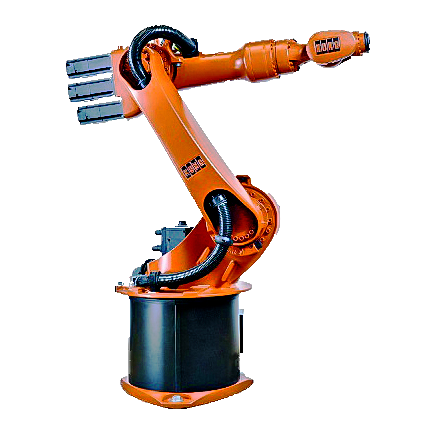
\includegraphics[scale=0.45]{6R.png}
    \end{minipage}
\end{figure}

 \pause \item \begin{figure}[!ht] les logiciels assistants de preuve (Coq) \begin{minipage}[c]{.3\linewidth}
        \centering
        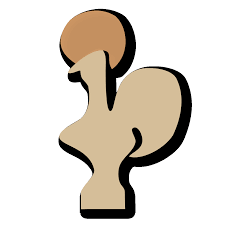
\includegraphics[scale=0.18]{logoCoq.png}
    \end{minipage}
\end{figure}

\pause \item \begin{figure}[!ht] les algèbres géométriques \begin{minipage}[c]{.3\linewidth}
        \centering
        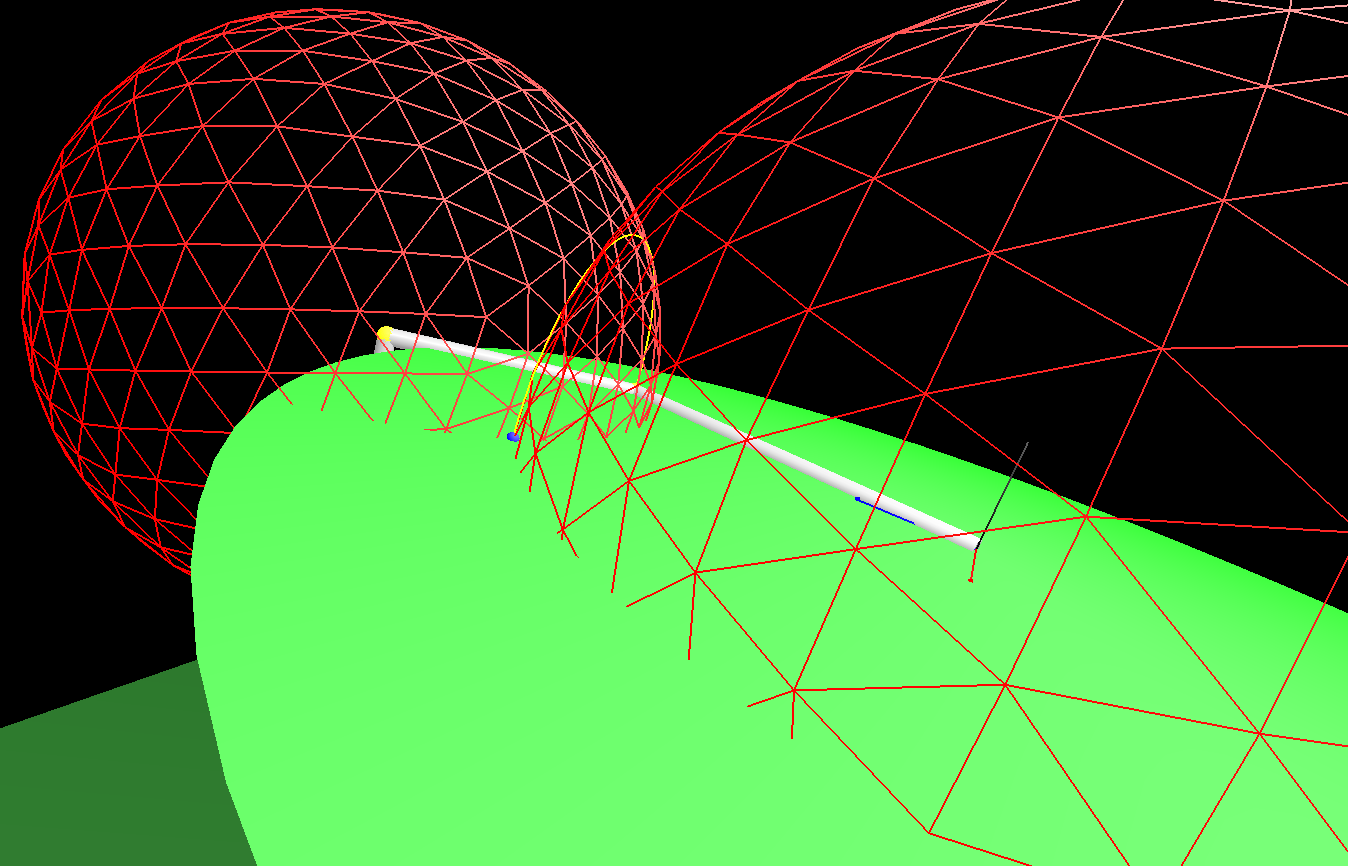
\includegraphics[scale=0.07]{SCARAIK2.png}
    \end{minipage}
\end{figure}

\end{itemize}

\end{frame}



\subsection{Les logiciels assistants de preuve}
\frame{
\frametitle{Les logiciels assistants de preuve}
\pause
Le but d'un logiciel assistant de preuve est de prouver un théorème mathématique ou les lignes de code composant un programme, c'est-à-dire que les lignes de code exécutent bien ce qui est attendu.

\pause \sg{Avantage} : le programme fait ce qu'il doit faire et ne plante pas.\vspace{0.1cm}\pause

Exemple : Le vol 501 de la fusée Ariane a explosé en vol à cause d'un problème de dépassement d'entier. Le code du système de navigation n'était pas prouvé.  \begin{figure}[!ht]
\centering
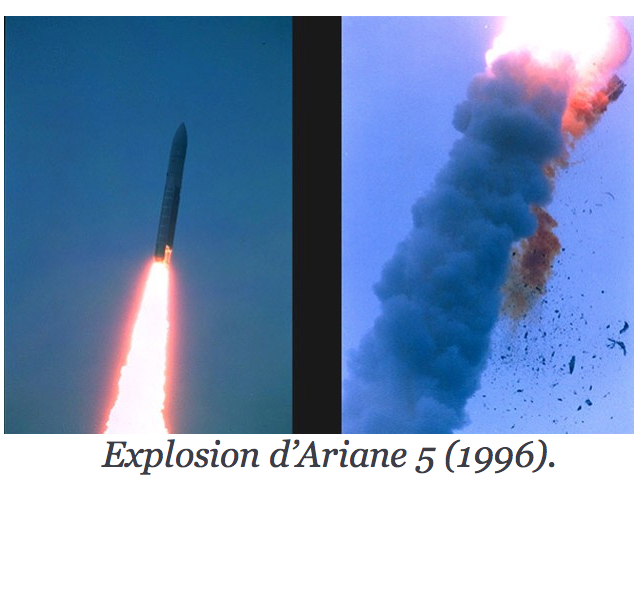
\includegraphics[scale=0.16]{ariane.png}
\end{figure}
}
\frame{
\frametitle{Les logiciels assistants de preuve}
 \sg{Inconvénient} : c'est très long ! On limite donc en général au maximum ce qui doit être prouvé et il faut trouver un formalisme adapté au problème\vspace{0.5cm}
}
\frame{

\frametitle{Les logiciels assistants de preuve}

Plusieurs théorèmes mathématiques ont été prouvés en utilisant des logiciels assistants de preuve, parmi eux :
\begin{itemize}
\item Le théorème des quatre couleurs en 2005
\item Le théorème de Feit-Thompson (tout groupe fini d'ordre impair est résoluble) en 2012 (plus de 6 ans pour 10 chercheurs)
\item La conjecture de Kepler (empilement optimal de sphères) en 2014
\end{itemize}
\pause
Des logiciels ont aussi été prouvés :
\begin{itemize}
\item  un compilateur C (CompCert) où il est prouvé que le code compilé se comporte comme le code source
\end{itemize}
 }
 
 \subsection{Les algèbres géométriques}

\begin{frame}
\frametitle{Les algèbres géométriques}
\pause
Les algèbres géométriques servent à représenter les éléments de la géométrie classique de façon plus uniforme. 
\pause \\
Un unique objet, \sg{le multivecteur} représente : 
\begin{itemize}
\item les points
\item les vecteurs
\item les plans
\item les droites
\item les sphères
\item les cercles 
\item les rotations
\item les translations...
\end{itemize}

\end{frame}

\frame{
\frametitle{Les algèbres géométriques}
Autre avantage : les cas particuliers n'existent pas.\bigskip


Par exemple le calcul permettant d'obtenir un plan à partir de deux vecteurs renverra $0$ si les deux vecteurs sont colinéaires.}

\frame{
Les algèbres géométriques ont été découvertes en 1844 par Grassmann puis formalisées par Clifford en 1873. Elles ont ensuite été oubliées jusque dans les années 1950 où Hestenes montrera que ces algèbres sont parfaitement adaptées pour résoudre des problèmes de relativité en dimension 4, d'électromagnétisme, ou de mécanique classique ou quantique. 

\pause Elles sont aujourd'hui utilisées en : 
\begin{itemize}
\item physique 
\item biomécanique
\item dynamique des vols spatiaux
\item vision par ordinateur
\item robotique 
\end{itemize}
}

\section{Les algèbres géométriques}

\subsection{Multivecteurs}
\frame{

\frametitle{Les algèbres géométriques}
L'algèbre géométrique $\mathscr{G}^n$ peut être vue comme une extension de l'espace vectoriel $\R^n$.\pause

Les objets de cet algèbre sont appelés \sg{multivecteurs}. \pause

L'algèbre $\mathscr{G}^n$ possède plusieurs opérations :
\begin{itemize}
\item une somme prolongeant la somme classique des vecteurs\pause
\item un produit appelé produit géométrique, noté $ab$ pour deux multivecteurs $a$ et $b$\pause
\item un produit scalaire (et donc une norme) noté $a \cdot b$\pause
\item un produit extérieur noté $a \wedge b$
\end{itemize}
}

\frame{
\frametitle{Les algèbres géométriques}
Si $\lbrace \bm{e_1},\cdots, \bm{e_n} \rbrace$ est une base orthonormée de $\R^n$, les éléments $\boldsymbol{e_i} \mathbf{e_j}$ appartiennent donc à $\mathscr{G}^n$, mais ne sont pas des vecteurs de $\R^n$.\vspace{0.5cm}
\pause 

$dim(\mathscr{G}^n) = 2^n$, une base étant formée par $1$ et l'ensemble des produits de vecteurs distincts : 
$$\lbrace 1, \bm{e_1}, \cdots, \bm{e_n}, \bm{e_1} \bm{e_2}, \bm{e_1}  \bm{e_3}, \cdots \bm{e_{n-1}} \bm{e_n}, \bm{e_1} \bm{e_2}  \bm{e_3}, \cdots, \bm{e_1}\cdots \bm{e_n}\rbrace$$
\bigskip
L'élément $\bm{\bm{e_i}\bm{e_j}}$ sera noté par la suite $e_{ij}$.
}
\subsection{Interprétation géométrique des bivecteurs}
\begin{frame}
\frametitle{Les algèbres géométriques - Interprétation géométrique}
\pause
  En 1D :  un vecteur définit une droite et sa norme est la longueur d'un segment de cette droite, et il possède un sens.\vspace{6.5cm}
\end{frame}
   
\begin{frame}
\frametitle{Les algèbres géométriques - Interprétation géométrique}
 En 2D : Si $\bm{u}$ et $\bm{v}$ sont des vecteurs (non colinéaires), $\bm{u}\wedge \bm{v}$ est appelé un \sg{bivecteur}.\bigskip \pause
   \begin{figure}[!ht]
\centering
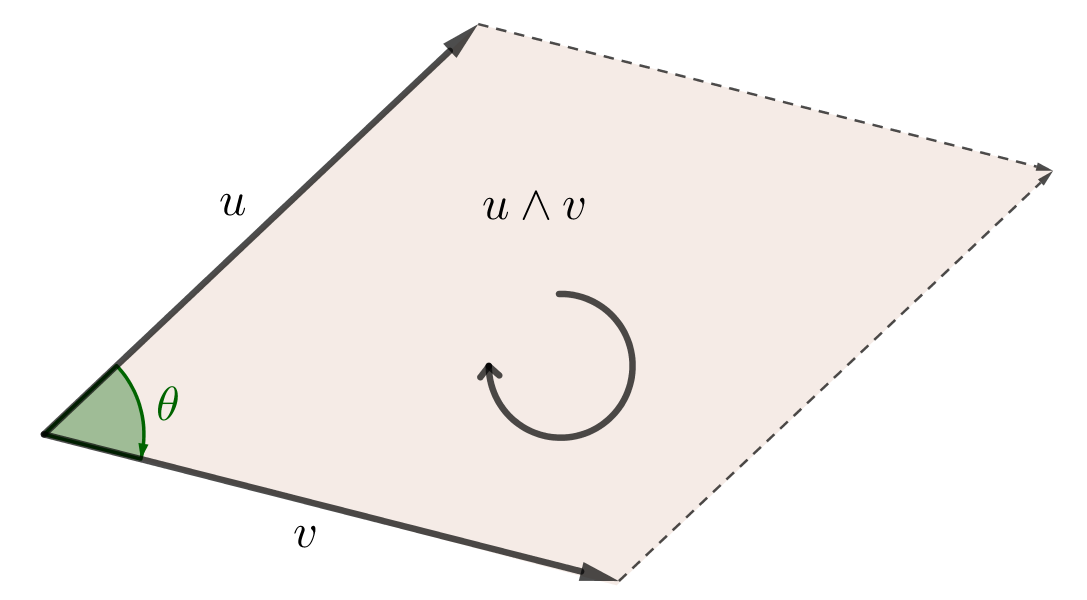
\includegraphics[scale=0.115]{bivecteur.png}
\end{figure}
Un bivecteur $\bm{u} \wedge \bm{v}$ \begin{itemize}
\item définit le plan vectoriel engendré par $\bm{u}$ et $\bm{v}$ \pause 
\item sa norme est une partie de l'aire de ce plan : c'est l'aire du parallélogramme engendré par $\bm{u}$ et $\bm{v}$ \pause 
\item possède également une orientation : celle de $\bm{u}$ vers $\bm{v}$
\end{itemize}
\end{frame}
   
\subsection{Egalité des bivecteurs}
\begin{frame}
\frametitle{Egalité de bivecteurs}
Deux vecteurs sont égaux s'ils ont même direction, même sens et même norme. \pause 

Deux bivecteurs sont égaux si et seulement si ils définissent le même plan, ont la même orientation et ont la même norme. \pause 

Ainsi, ces bivecteurs-là sont par exemple égaux : 

\begin{figure}[!ht]
\centering
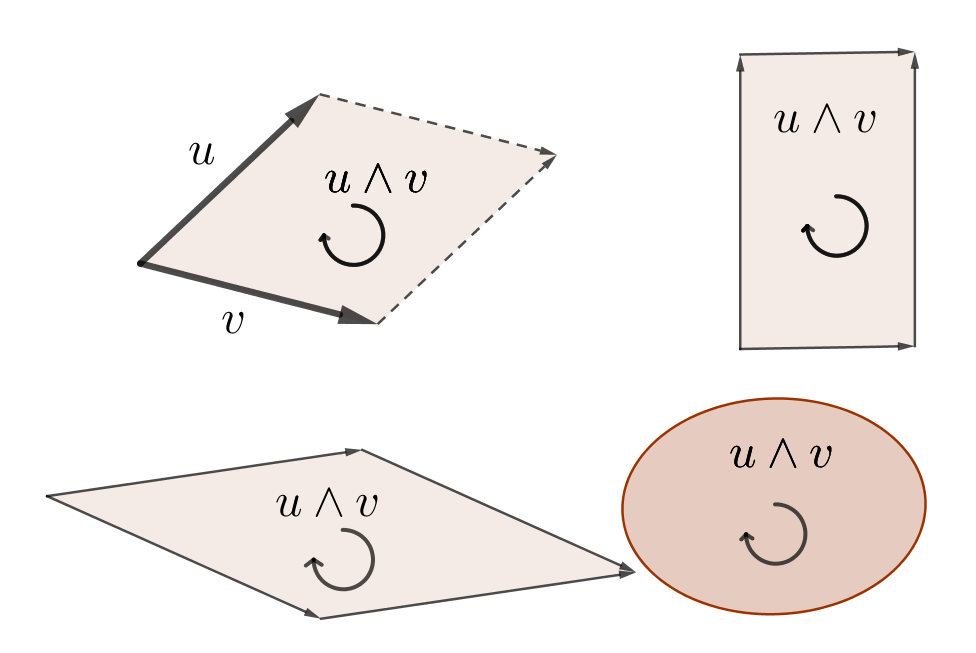
\includegraphics[scale=0.17]{egalite.png}
\label{egalite}
\end{figure}   
\end{frame}

\subsection{Addition de bivecteurs}
\begin{frame}
\frametitle{Addition de bivecteurs}
\pause
\begin{center}
{\sg{Etape 1}} 
\end{center}
\begin{figure}[!ht]
\centering
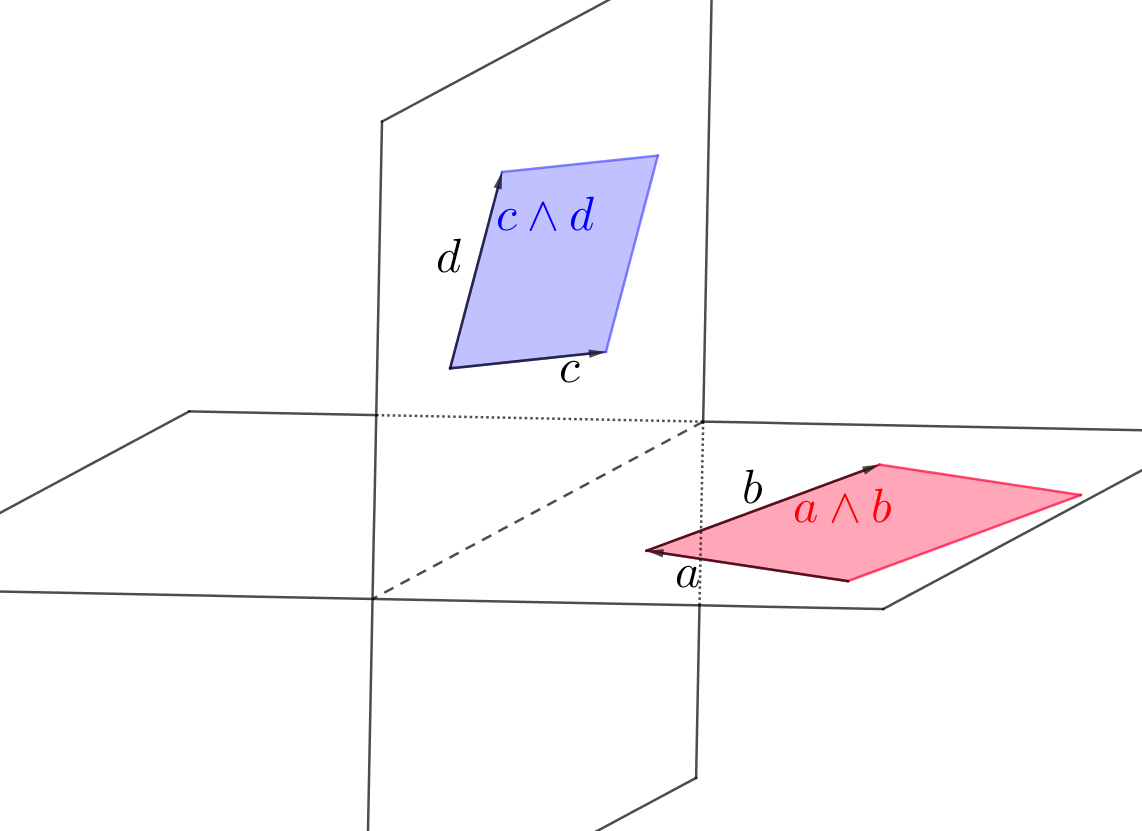
\includegraphics[scale=0.2]{1.png}
\end{figure}   
\end{frame}

\begin{frame}
\frametitle{Addition de bivecteurs}
\begin{center}\sg{Etape 2}  : on ramène les bivecteurs de sorte qu'ils aient un vecteur en commun
\end{center} 
\begin{figure}[!ht]
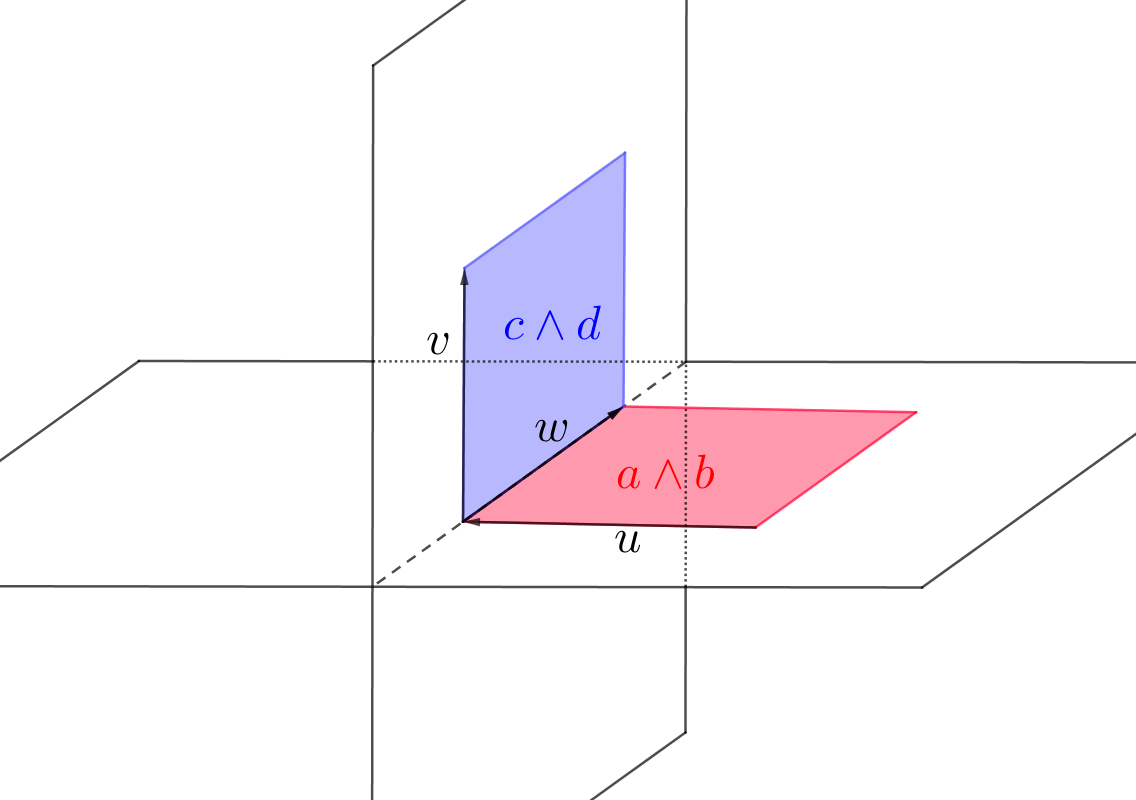
\includegraphics[scale=0.2]{2.png}
\end{figure}   
\end{frame}

\begin{frame}
\frametitle{Addition de bivecteurs}
\begin{center}
\sg{Etape 3}: par linéarité, le résultat est $(\bm{u}+\bm{v})\wedge\bm{w}$
\end{center}
\begin{figure}[!ht]
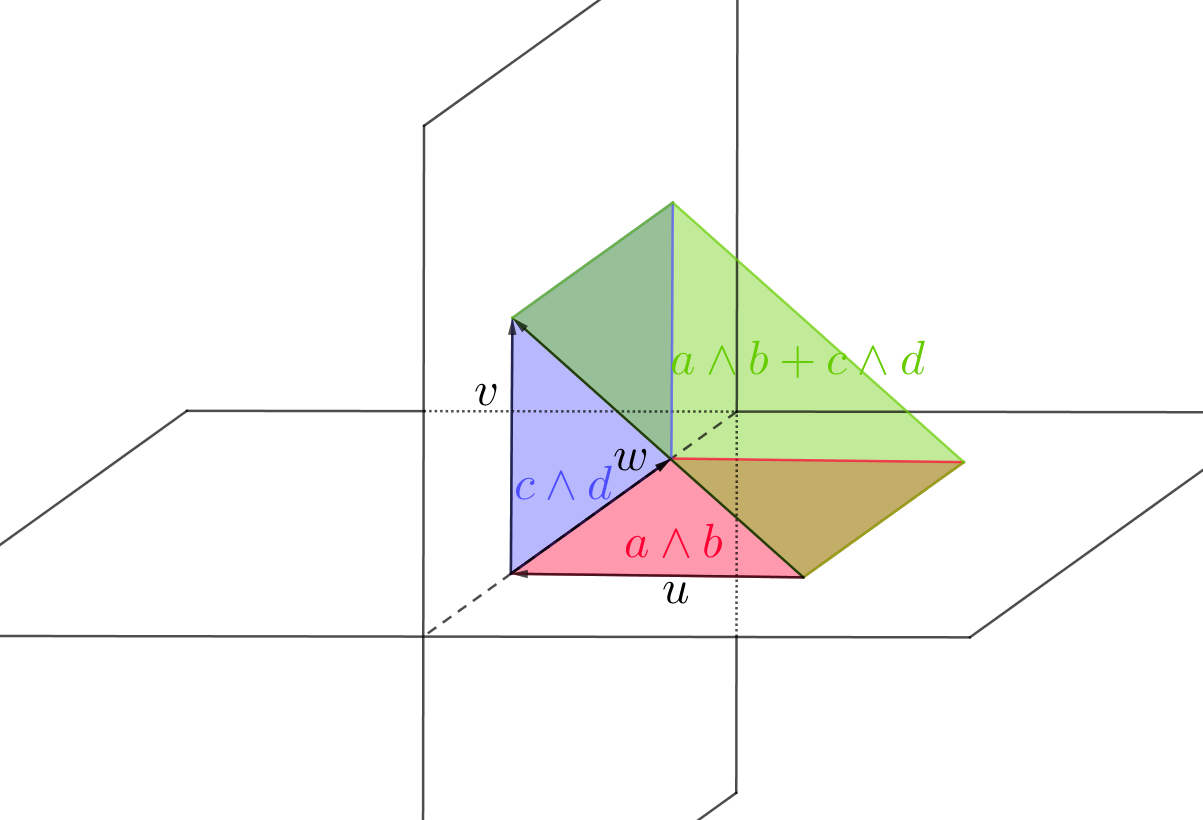
\includegraphics[scale=0.2]{3.png}
\end{figure}   
\end{frame}

\subsection{Trivecteurs}
\begin{frame}
\frametitle{Trivecteurs}

Tout ceci peut être prolongé à la notion de trivecteurs, quadrivecteurs, ...
\begin{figure}[!ht]
\centering
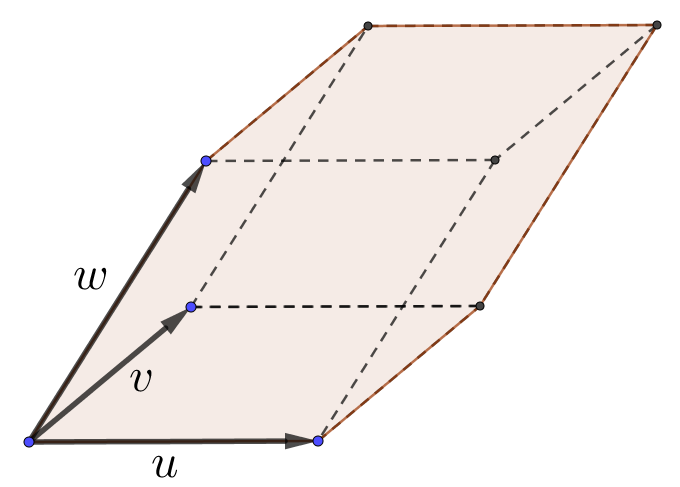
\includegraphics[scale=0.2]{trivecteur.png}
\end{figure}   
\end{frame}

\subsection{Lames - multivecteurs}
\begin{frame}
\frametitle{Lames - multivecteurs}
Une \sg{k-lame} est un multivecteur $\bm{A}$ de la forme $$\bm{A} = \bm{a_1}  \wedge \bm{a_2} \wedge \cdots \wedge \bm{a_k}$$ où les vecteurs  $\bm{a_1}, \cdots \bm{a_k}$ sont linéairement indépendants. 
\pause

Les 0-lames sont les constantes réelles, les 1-lames les vecteurs, les bivecteurs sont les 2-lames, les trivecteurs les 3-lames... 
\pause

Le grade maximal est $n$ : il n'y a qu'une $n$-lame (à une constante près) : $\bm{e_1} \wedge \cdots \wedge \bm{e_n}$. 

Cette lame est notée $I$ et est appelée \sg{pseudo-scalaire}.
\pause

Un \sg{multivecteur} sous sa forme générale est donc une somme de lames de grades différents.

 Par exemple, dans $\mathscr{G}^3$, $2+ \bm{e_1}-3\bm{e_3}+2e_{12}-4e_{123}$ est un multivecteur.
\end{frame}

\subsection{Réversion, inverse et dual}
\begin{frame}
\frametitle{Réversion, inverse et dual}
Si $\bm{A} = \bm{a_1}  \wedge \bm{a_2} \wedge \cdots \wedge \bm{a_k}$, on appelle réversion de $\bm{A}$, notée $\tilde{\bm{A}}$ la lame $$\tilde{\bm{A}} =  \bm{a_k} \wedge \cdots \wedge \bm{a_1}$$


Ceci sert à montrer que les lames sont inversibles et à construire leur inverse, car $\tilde{\bm{A}}$ et $\bm{A^{-1}}$ sont égaux à une constante près. 
\pause

Mais un multivecteur en général n'a pas d'inverse ! Les algèbres ne sont pas des corps. 

\pause
Le dual d'un multivecteur $A$ est le multivecteur $$A^* = AI^{-1}$$
Il représente tout l'espace non pris par $A$.
\pause

Par exemple, dans $\mathscr{G}^3$, on a $\bm{e_{1}}^* =  -\bm{e_2} \wedge \bm{e_3}$.

\end{frame}

\section{Algèbre géométrique conforme (CGA)}
\subsection{Présentation}
\begin{frame}
\frametitle{CGA - Présentation}
\pause
On se place dans $\mathscr{G}^{4,1}$, l'algèbre géométrique formée à partir d'un espace de dimension 5 (donc de dimension $2^5=32$). 

Base orthogonale : $\bm{e_1}$, $\bm{e_2} $,  $\bm{e_3}$ , $\bm{e_+}$ et $\bm{e_-}$ avec  : 
$$||\bm{e_+}|| = 1 \text{ et } ||\bm{e_-}|| = -1$$ \pause

En pratique, on utilisera plutôt les vecteurs $\bm{e_0}$ et $\ei$ définis par : 
$$ \bm{e_0} = \frac{1}{2} (\bm{e_-} - \bm{e_+}) \text{ et }  \ei = \bm{e_+}+ \bm{e_-}$$
car plus parlant : 

$\bm{e_0}$ représente l'origine du repère et $\ei$ représente un point à l'infini.

\end{frame}

\begin{frame}
\frametitle{Passage d'un point 3D à des coordonnées CGA}
A $\bm{x}$ de coordonnées $(a,b,c)$ dans une base donnée de $\R^3$, on associe le vecteur CGA par la formule : $x = a \bm{e_1} + b \bm{e_2} + c \bm{e_3} + \bm{e_0} + \frac{1}{2}||\bm{x}||^2 \ei$, ce qui s'écrit aussi : 

$$x = \bm{x} + \bm{e_0} + \frac{1}{2}||\bm{x}||^2 \ei$$

\end{frame}
\begin{frame}
\frametitle{Représentations IPNS et OPNS}
On cherche maintenant à représenter d'autres espaces que des points.\pause

On a deux représentations possibles, duales l'une de l'autre : 
\begin{itemize}
\item l'IPNS consiste à dire que le multivecteur $x$ correspond à notre espace $E$ si $$\forall y \text{ vecteur de } \mathscr{G}^{4,1}, y\in E \Leftrightarrow x \cdot y =0.$$\pause
\item l'OPNS consiste à dire que le multivecteur $x$ correspond à notre espace $E$ si $$\forall y \text{ vecteur de } \mathscr{G}^{4,1}, y\in E \Leftrightarrow x \wedge y =0.$$
\end{itemize}
\end{frame}

\begin{frame}
\begin{table}[h!]
\begin{center}

\begin{tabular}{|c|c|c|c|}
\hline

Objets & Représentation IPNS &  Représentation OPNS  \\\hline
Point $x$ & $x = \bm{x} + \bm{e_0} + \frac{1}{2}||\bm{x}||^2 \ei$ & $x^* = s_1 \wedge s_2 \wedge s_3 \wedge s_4$  \\
\hline

Sphère $s$ &  $s = \bm{c} + \frac{1}{2}(\bm{c}^2-r^2)\ei + \ez$ &  $s^* = a \wedge b \wedge c \wedge d$  \\
\hline

Plan $P$ &  $P = \bm{n} + d\ei$ &  $P^* = a \wedge b \wedge c \wedge \ei$  \\
\hline

Droite $D$  &  $D = P_1 \wedge P_2$ & $D^* = a \wedge b \wedge \ei$  \\\hline

Cercle $c$  & $c = s_1 \wedge s_2$  & $c^* = a \wedge b \wedge c$  \\
\hline

Paire de  &  $P_p = s_1 \wedge s_2 \wedge s_3 $ & $P_p^* = a \wedge b$  \\
points $P_p$ & &\\\hline
\end{tabular}
\end{center}
\renewcommand{\thetable}{\arabic{table}}
\end{table}
\end{frame}

\begin{frame}
\frametitle{Transformations}
\begin{itemize}
\item Pour une rotation d'angle $\theta$ de plan ayant $\bm{n}$ comme vecteur normal, on note $$R = cos\left(\frac{\theta}{2}\right)- sin\left(\frac{\theta}{2}\right) \bm{n} \text{\hspace*{1cm} (appelé \sg{rotor})}$$ 

L'image du multivecteur $X$ par cette rotation est $RX\tilde{R}$.\pause
\item Pour une translation de vecteur $\bm{t}$, on note $$T = 1-\frac{1}{2} \bm{t} \ei $$ L'image du multivecteur $X$ par cette translation est $TX\tilde{T}$.
\end{itemize}
\end{frame}

\section{Le logiciel Coq}

\begin{frame}
\frametitle{Présentation de Coq}
Pour voir rapidement le fonctionnement de Coq, nous allons regarder la démonstration de la formule : 

$$\sum_{k=0}^n k = \frac{n(n+1)}{2}$$
\end{frame}

\section{Robots en algèbres géométriques en Coq}
\subsection{Algèbres géométriques conformes}
\begin{frame}
\frametitle{Implémentation de la CGA}
\pause

\textbf{Première partie :} 

On implémente les algèbres géométriques conformes en Coq en réutilisant les bibliothèques de Laurent Théry.\bigskip
\pause

\textbf{Deuxième partie :} 

On définit des fonctions qui créent en Coq les différents objets géométriques vus plus haut dans le tableau.\bigskip

\end{frame}

\begin{frame}
\frametitle{Implémentation de la CGA}
\vspace{-0.8cm}
\begin{figure}[!ht]
\hspace*{-1.1cm}
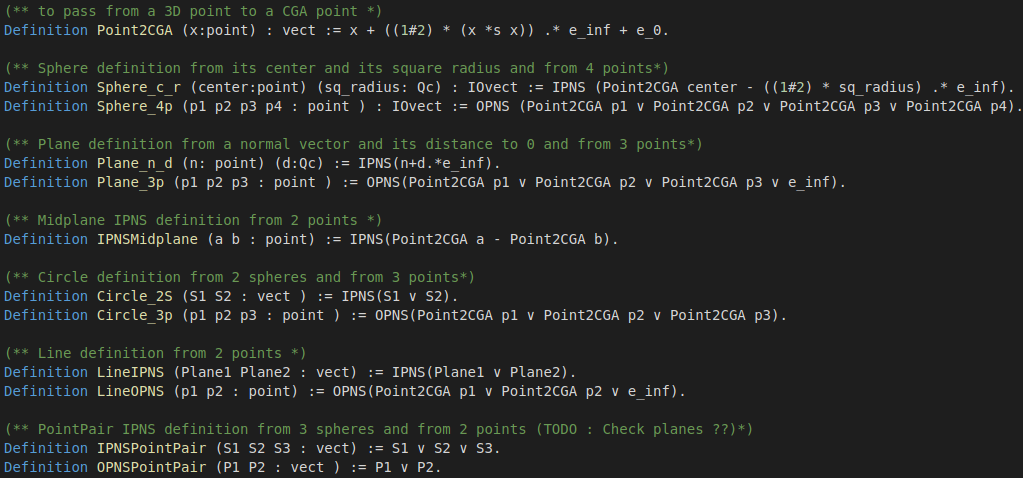
\includegraphics[scale=0.4]{cga2.png}
\end{figure}
\end{frame}

\begin{frame}
\begin{table}[h!]
\begin{center}

\begin{tabular}{|c|c|c|c|}
\hline

Objets & Représentation IPNS &  Représentation OPNS  \\\hline
Point $x$ & $x = \bm{x} + \bm{e_0} + \frac{1}{2}||\bm{x}||^2 \ei$ &   \\
\hline

Droite $D$  & & $D^* = a \wedge b \wedge \ei$  \\\hline

\end{tabular}
\end{center}
\renewcommand{\thetable}{\arabic{table}}
\end{table}
\begin{figure}[!ht]
\hspace*{-0.6cm}
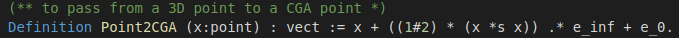
\includegraphics[scale=0.5]{Point2CGA.png}
\end{figure}
\begin{figure}[!ht]
\hspace*{-0.6cm}
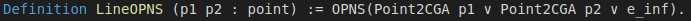
\includegraphics[scale=0.5]{LineOPNS.png}
\end{figure}
\end{frame}

\begin{frame}
\frametitle{Implémentation de la CGA}

Ensuite, on définit la fonction suivante, qui vérifie si un point vérifie les propriétés d'appartenance à un objet en CGA : 

\begin{figure}[!ht]
\hspace*{-1.1cm}
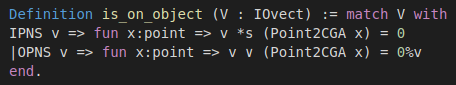
\includegraphics[scale=0.6]{cga3.png}
\end{figure}
\pause

Et on démontre plusieurs lemmes comme celui-ci : 
\begin{figure}[!ht]
\hspace*{-0.6cm}
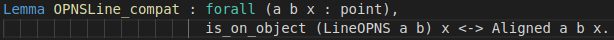
\includegraphics[scale=0.55]{Lemma.png}
\end{figure}
(où la fonction $Aligned$ est la fonction qui nous dit si trois points en géométrie classique sont alignés) 
\end{frame}


\subsection{Cinématique directe}
\begin{frame}
\frametitle{Cinématique directe}

En robotique, la cinématique directe consiste pour un bras de robot donné à pouvoir calculer où se situera le bout du bras, appelé \sg{effecteur}, en fonction des paramètres d'entrée.\pause\bigskip

Dans cette partie, nous avons créé trois robots, implémenté une fonction cinématique directe à l'aide des algèbres géométriques, et observé graphiquement les résultats obtenus. Je vais en présenter un seul ici : le robot 6R.
\end{frame}


%\begin{frame}
%\frametitle{Cinématique directe - Préliminaires}
%Le but est de créer les multivecteurs des rotors et les translations définies plus haut. 
%
%On définit donc les rotors et les translations, puis les transformations en général comme ceci : \pause
%\begin{figure}[!ht]
%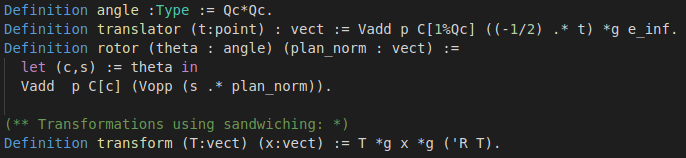
\includegraphics[scale=0.5]{robot1.png}
%\end{figure}
%
%\end{frame}

\begin{frame}
\frametitle{Robot 6R}
Un robot 6R est un robot ayant 6 axes de rotation. Il est constitué d'une base et d'une partie plus petite appelée "poignet".

\begin{figure}[!ht]
    \begin{minipage}[c]{.46\linewidth}
        \centering
        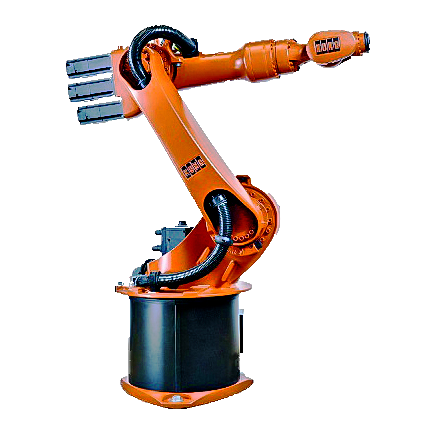
\includegraphics[scale=1.4]{6R.png}
    \end{minipage}
    \hfill%
    \begin{minipage}[c]{.46\linewidth}
        \centering
        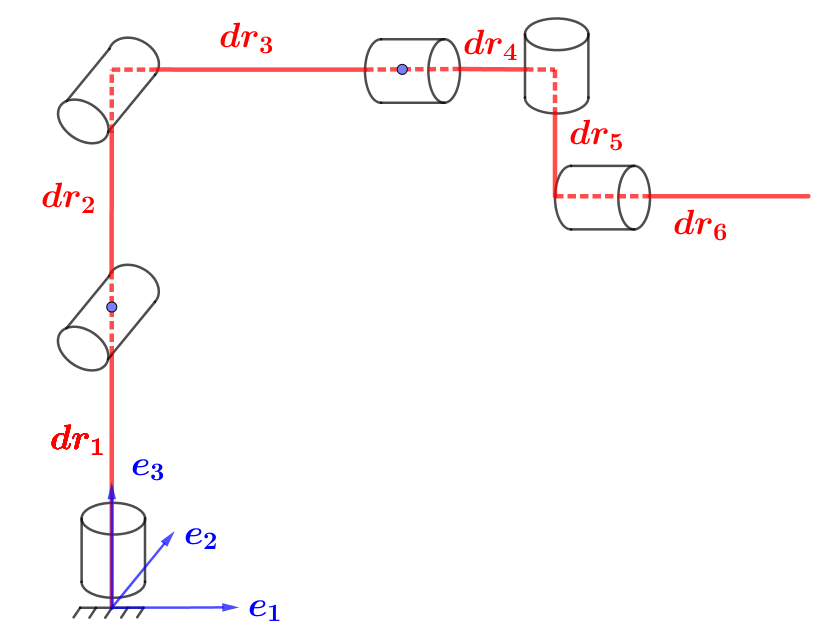
\includegraphics[scale=0.2]{6RGeo.png}
    \end{minipage}
\end{figure}

\end{frame}
\begin{frame}
\frametitle{Robot 6R}
On crée les paramètres du robot : 
\begin{figure}[!ht]
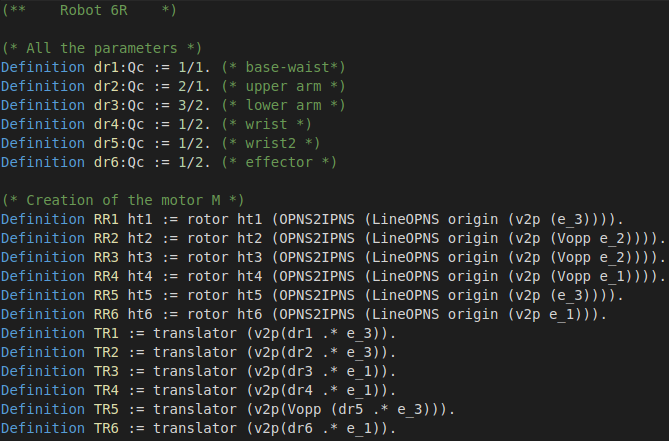
\includegraphics[scale=0.37]{6RParam.png}
\end{figure}

\end{frame}

\begin{frame}
\frametitle{Robot 6R}
Et on lui fait calculer la position finale de l'effecteur (la fonction $effector$ calcule l'image par la transformation $robot6R$ de l'origine) \vspace{-0.4cm}
\begin{figure}[!ht]
\hspace*{-0.7cm}
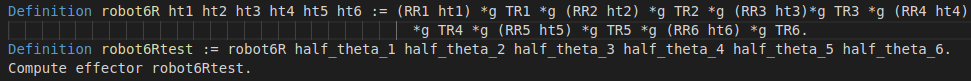
\includegraphics[scale=0.36]{6RDef.png}
\end{figure}\vspace{-0.3cm}

On trouve, pour des valeurs d'angles choisies au hasard : 

\begin{figure}[!ht]
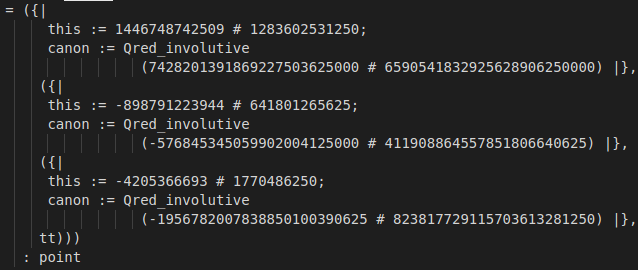
\includegraphics[scale=0.3]{6RRes.png}
\end{figure} soit à peu près $(1.13, −1.40, −2.38)$.
\end{frame}

\begin{frame}
\frametitle{Robot 6R}
On peut voir le résultat graphiquement sur le logiciel CLUCalc : 

\begin{figure}[!ht]
    \begin{minipage}[c]{.46\linewidth}
        \centering
        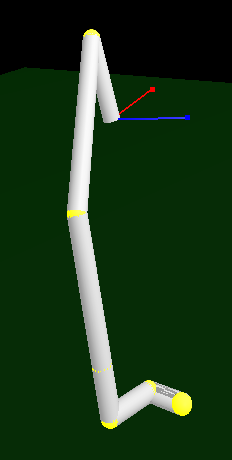
\includegraphics[scale=0.45]{6RCluCalc.png}
    \end{minipage}
    \hfill%
    \begin{minipage}[c]{.46\linewidth}
        \hspace*{-1.5cm}
        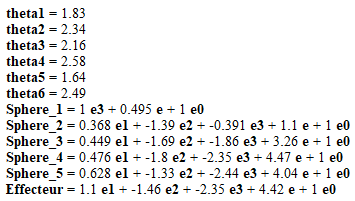
\includegraphics[scale=0.75]{6RCluRes.png}
    \end{minipage}
\end{figure}
\end{frame}


\subsection{Cinématique indirecte}

\begin{frame}
\frametitle{Cinématique indirecte}
La cinématique indirecte consiste à prendre le problème dans le sens inverse : on choisit un endroit où doit se situer l'effecteur et on cherche quels paramètres rentrer dans le robot pour y arriver.\bigskip \pause

Il peut y avoir plusieurs problèmes : 
\begin{itemize}
\item le point choisi n'est pas atteignable
\item il y a plusieurs façons d'arriver au point choisi 
\item il y a une infinité de façons d'arriver au point choisi
\end{itemize}
\pause
Dans cette partie, on va montrer comment trouver des solutions au problème pour le robot SCARA.

\end{frame}

\begin{frame}
\frametitle{Robot SCARA}

Voici le robot SCARA, ainsi que ses liaisons schématiques : 

\begin{figure}[!ht]
    \begin{minipage}[c]{.46\linewidth}
        \centering
        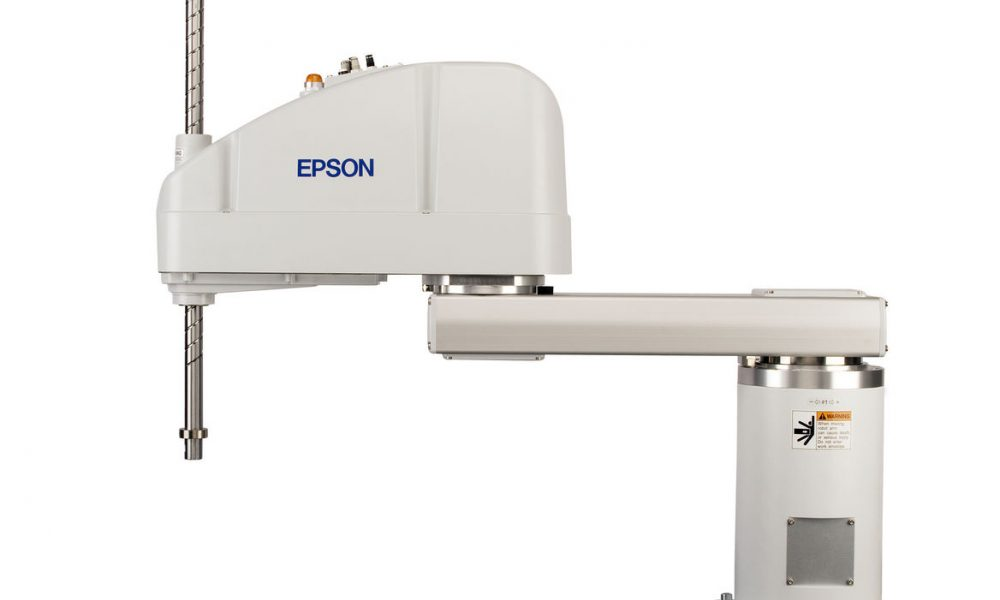
\includegraphics[scale=0.17]{Scara.jpg}
    \end{minipage}
    \hfill%
    \begin{minipage}[c]{.46\linewidth}
        \centering
        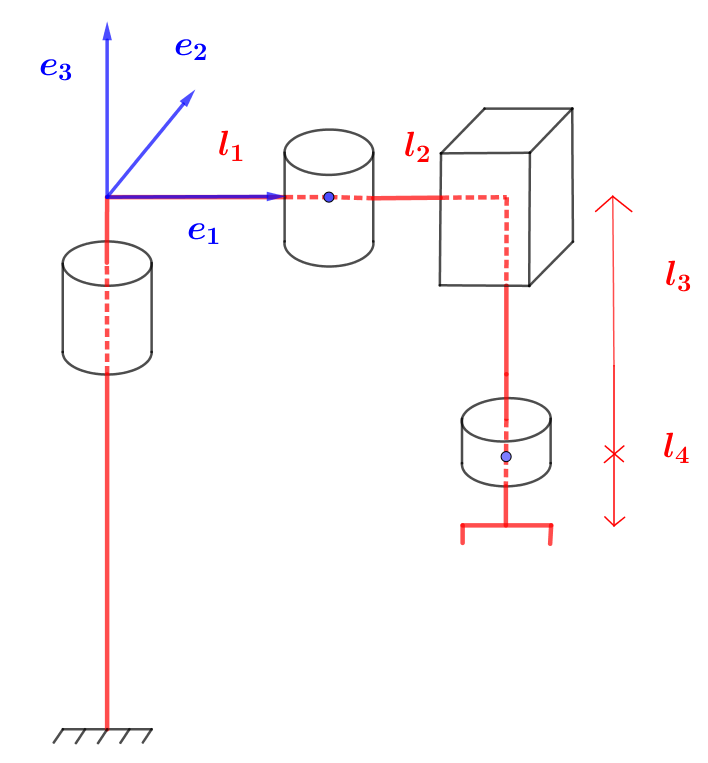
\includegraphics[scale=0.2]{Scara.png}
    \end{minipage}
\end{figure}

\end{frame}

\begin{frame}
\frametitle{Robot SCARA}

Vu de dessus, l'ensemble des points atteignables est colorié en rouge. Pour la cote, cela ne dépend que de la translation du bras.

\begin{figure}[!ht]
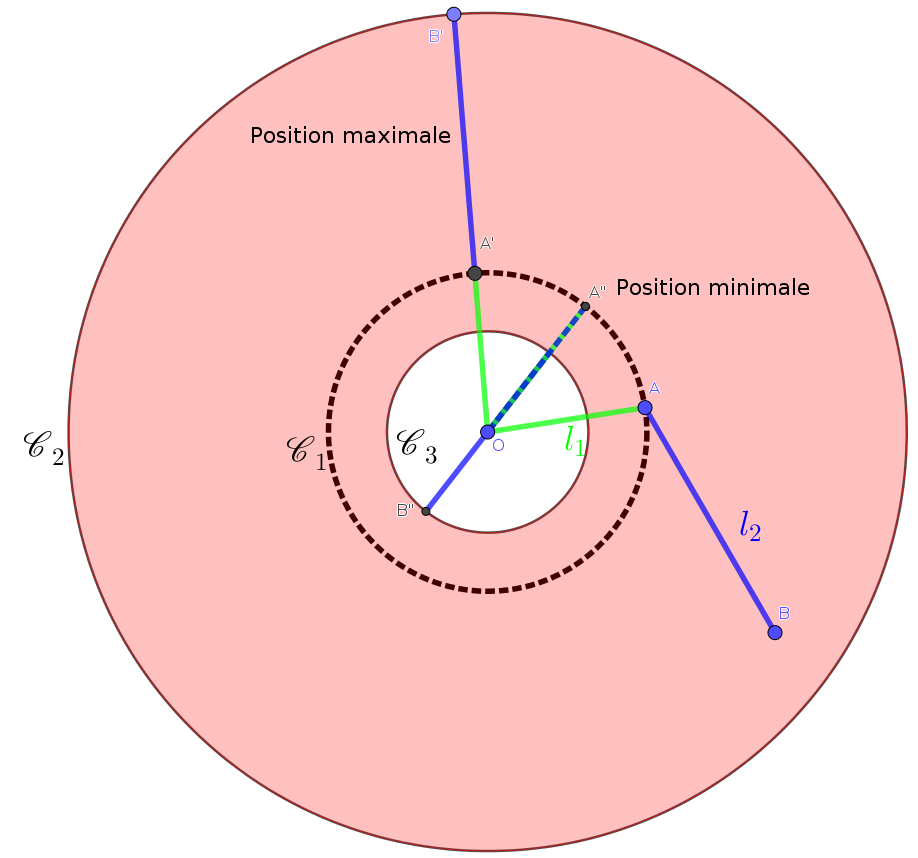
\includegraphics[scale=0.175]{SCARADessus.png}
\end{figure}
\end{frame}

\begin{frame}
\frametitle{Robot SCARA}
Si un point est strictement compris dans l'anneau rouge au-dessus, il y aura toujours deux façons d'atteindre le point considéré : 

\begin{figure}[!ht]
\centering
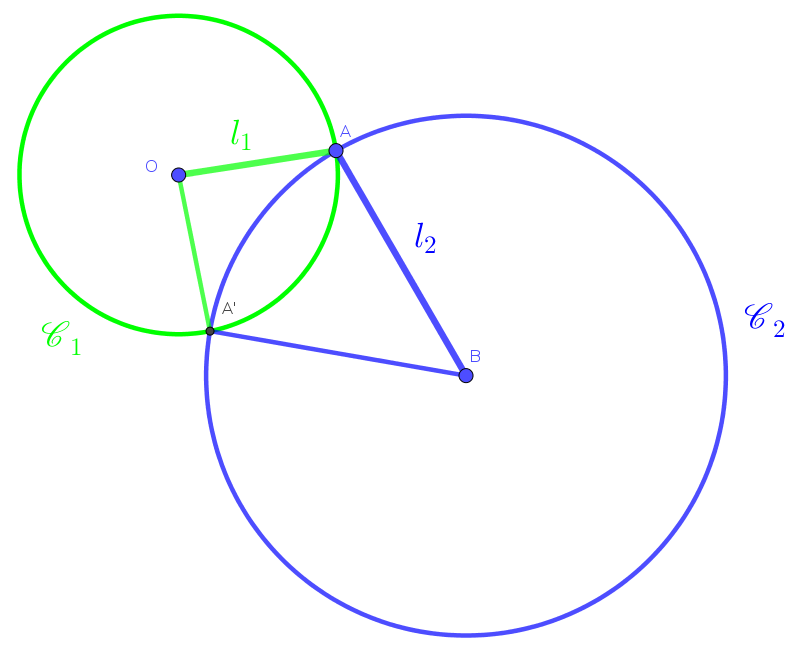
\includegraphics[scale=0.22]{SCARADessus2.png}
\end{figure}
\end{frame}

\begin{frame}
\frametitle{Robot SCARA}


Avec les algèbres géométriques, on cherche la position du point $A$, intersection des deux bras.


Pour cela, on remarque que : 
\end{frame}

\begin{frame}
\begin{figure}[!ht]
\includegraphics[scale=0.25]{ScaraIK.png}
\end{figure}
\end{frame}

\begin{frame}
\frametitle{Robot SCARA}
On note $B$ le point extrémité du deuxième bras : $B(x,y,0)$

Pour calculer ces points avec les algèbres géométriques, on cherche la position du point $A$, intersection des deux bras.


Pour cela, on remarque que : 
\begin{itemize}
\item le point $A$ est sur le plan $P$ d'équation $z=0$. 
\item sa distance à $O$ est de $l_1$, donc il est situé sur la sphère $S_1$ de centre $O$ de rayon $l_1$. 
\item $A$ est situé à une distance de $l_2$ de $B$, donc il est sur la sphère $S_2$ de centre $B$ de rayon $l_2$. 
\end{itemize}


\end{frame}

\begin{frame}
\vspace*{-0.7cm}
\begin{figure}[!ht]
\hspace*{-1cm}
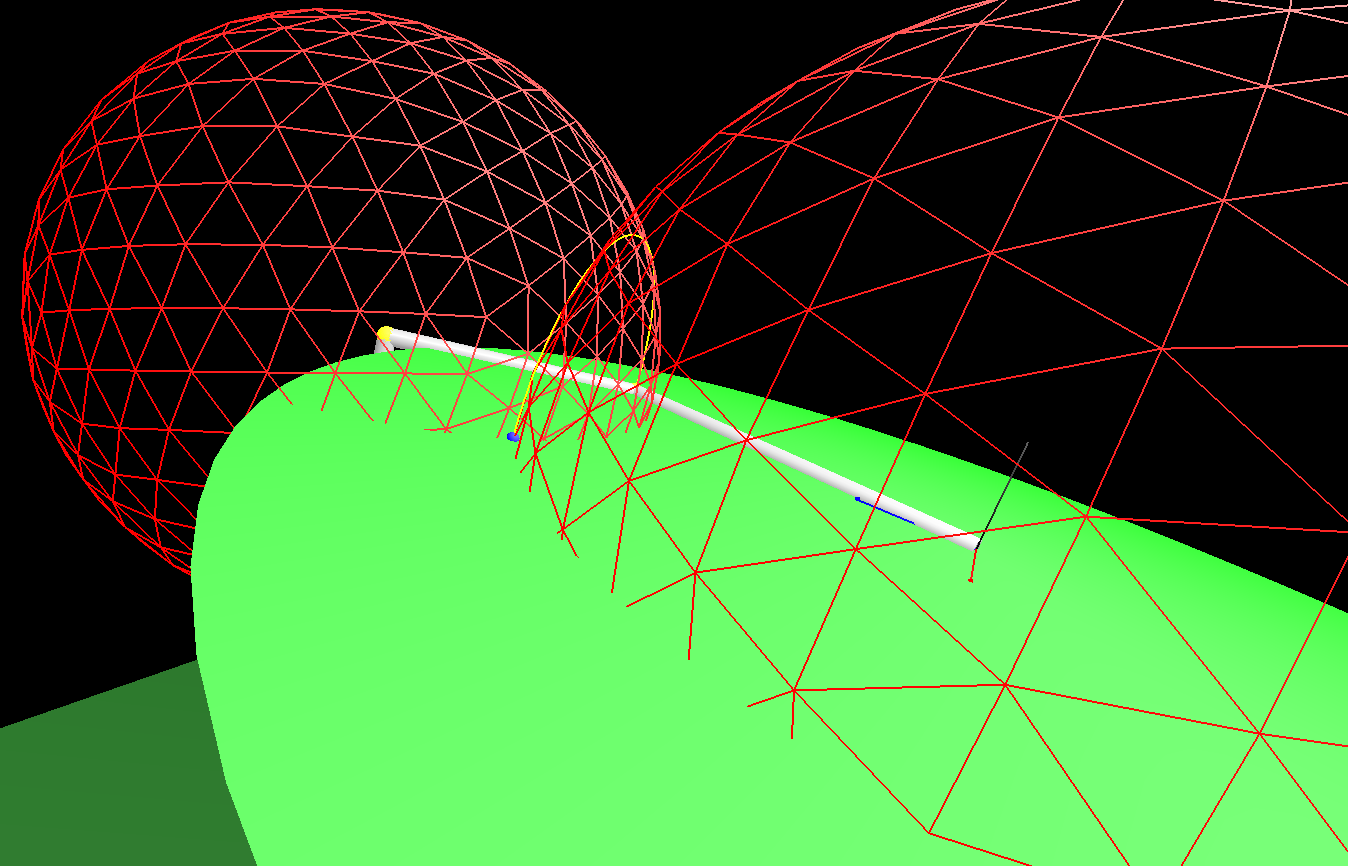
\includegraphics[scale=0.34]{SCARAIK2.png}
\end{figure}

\end{frame}

\begin{frame}

\frametitle{Robot SCARA}
Au final, pour avoir la position de $A$, il suffit de calculer $$P \wedge S_1 \wedge S_2$$

Cela renverra une paire de points, notée $P_p$. \pause

Pour extraire un seul point, il faut calculer $$\frac{Pp^* \pm \sqrt{Pp^* \cdot Pp^*} }{\ei \cdot Pp^*}$$
le signe choisi donnant un point ou l'autre. 


\end{frame}

\begin{frame}
\frametitle{Robot SCARA}

\begin{figure}[!ht]
    \begin{minipage}[c]{.46\linewidth}
        \centering
        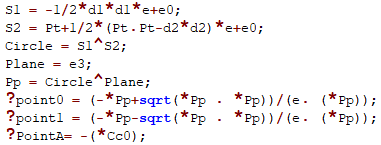
\includegraphics[scale=0.6]{SCARAIK3.png}
        \caption{Les calculs}
    \end{minipage}
    \hfill%
    \begin{minipage}[c]{.46\linewidth}
        \centering
        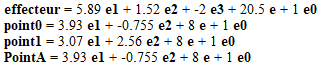
\includegraphics[scale=0.7]{SCARAIK4.png}
        \caption{Les résultats}
    \end{minipage}
\end{figure}



\end{frame}

\begin{frame}
Une fois les coordonnées du point $A$ connu, il ne reste qu'à utiliser les formules d'Al-Kashi :  
$$\theta_1 = arccos \left(\frac{l_1^2+OB^2-l_2^2}{2 l_1 OB}\right)\text{ et }\theta_2 = arccos \left(\frac{l_1^2+l_2^2-OB^2}{2 l_1 l_2}\right)$$

\begin{figure}[!ht]
\centering
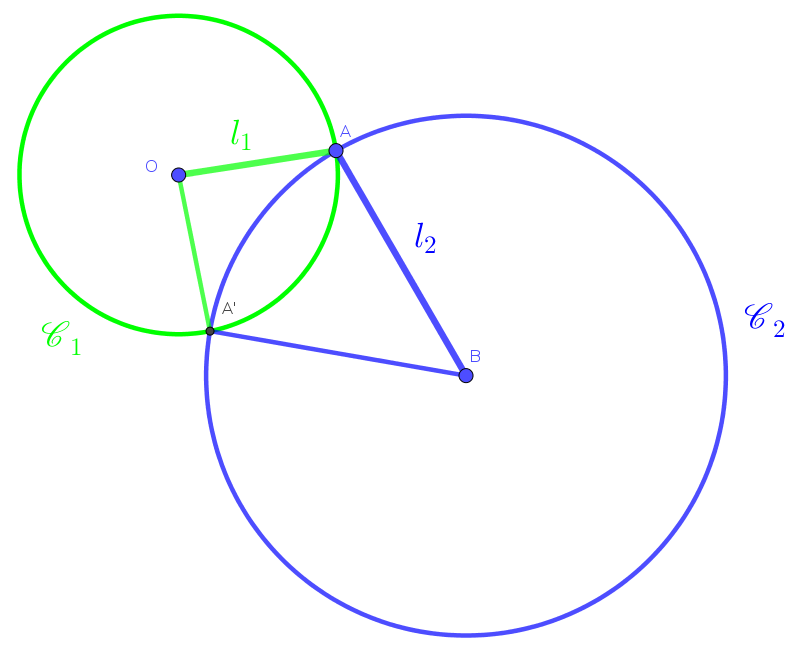
\includegraphics[scale=0.21]{SCARADessus2.png}
\end{figure}
\end{frame}
\section{Conclusion}
\begin{frame}
\frametitle{Difficultés rencontrées}
Pour pouvoir faire les calculs, le corps de base utilisé a été $\Q$. En effet, l'ensemble des nombres réels étant mathématiquement compliqué (l'ensemble des limites des suites de Cauchy), il est compliqué à manipuler en Coq (qui ne les remplace pas par des flottants), surtout pour faire des calculs. \pause \bigskip

Le problème, c'est qu'une fois dans $\Q$, le calcul des rotors $R = cos\left(\frac{\theta}{2}\right)- sin\left(\frac{\theta}{2}\right) \bm{n}$ pose problème à cause des fonctions trigonométriques.
\end{frame}

\begin{frame}
Pour contourner le problème, les angles ont été définis par leur cosinus et sinus comme des paires $(c,s)$ où $c$ et $s$ sont des rationnels. \pause \bigskip

Ce n'est en fait pas limitant, car on peut montrer que tout angle peut être limite d'une suite de tels angles.\pause \bigskip

Mais le problème réapparait dans les formules $$\frac{Pp^* \pm \sqrt{Pp^* \cdot Pp^*} }{\ei \cdot Pp^*} \text{ et } \theta_1 = arccos \left(\frac{l_1^2+OB^2-l_2^2}{2 l_1 OB}\right)$$ où les nombres irrationnels apparaitront immanquablement.
\end{frame}

\begin{frame}
\frametitle{Conclusion}

On a maintenant des robots dont les mouvements sont prouvés : il n'iront pas ailleurs que où il doivent aller. 
\pause\bigskip


Perspectives : \begin{itemize}
\item Finir d'implémenter la cinématique indirecte en Coq\pause
\item Prouver que la composée de la cinématique indirecte et directe donne bien l'identité\pause
\item Faire en sorte qu'un robot aille d'un endroit à un autre sans passer par une zone interdite (une artère par exemple)
\end{itemize} 

\end{frame}

\frame{\centering\textbf{\LARGE Merci pour votre attention !}}

\end{document}